\documentclass[bachelor, och, coursework]{SCWorks}
% параметр - тип обучения - одно из значений:
%    spec     - специальность
%    bachelor - бакалавриат (по умолчанию)
%    master   - магистратура
% параметр - форма обучения - одно из значений:
%    och   - очное (по умолчанию)
%    zaoch - заочное
% параметр - тип работы - одно из значений:
%    referat    - реферат
%    coursework - курсовая работа (по умолчанию)
%    diploma    - дипломная работа
%    pract      - отчет по практике
% параметр - включение шрифта
%    times    - включение шрифта Times New Roman (если установлен)
%               по умолчанию выключен
\usepackage{subfigure}
\usepackage{tikz,pgfplots}
\pgfplotsset{compat=1.5}
\usepackage{float}

%\usepackage{titlesec}
\setcounter{secnumdepth}{4}
%\titleformat{\paragraph}
%{\normalfont\normalsize}{\theparagraph}{1em}{}
%\titlespacing*{\paragraph}
%{35.5pt}{3.25ex plus 1ex minus .2ex}{1.5ex plus .2ex}

\titleformat{\paragraph}[block]
{\hspace{1.25cm}\normalfont}
{\theparagraph}{1ex}{}
\titlespacing{\paragraph}
{0cm}{2ex plus 1ex minus .2ex}{.4ex plus.2ex}

% --------------------------------------------------------------------------%


\usepackage[T2A]{fontenc}
\usepackage[utf8]{inputenc}
\usepackage{graphicx}
\graphicspath{ {./images/} }
\usepackage{tempora}

\usepackage[sort,compress]{cite}
\usepackage{amsmath}
\usepackage{amssymb}
\usepackage{amsthm}
\usepackage{fancyvrb}
\usepackage{listings}
\usepackage{listingsutf8}
\usepackage{longtable}
\usepackage{array}
\usepackage[english,russian]{babel}

% \usepackage[colorlinks=true]{hyperref}
\usepackage{url}

\usepackage{underscore}
\usepackage{setspace}
\usepackage{indentfirst} 
\usepackage{mathtools}
\usepackage{amsfonts}
\usepackage{enumitem}
\usepackage{tikz}
\usepackage{minted}

\newcommand{\eqdef}{\stackrel {\rm def}{=}}
\newcommand{\specialcell}[2][c]{%
\begin{tabular}[#1]{@{}c@{}}#2\end{tabular}}

\renewcommand\theFancyVerbLine{\small\arabic{FancyVerbLine}}

\newtheorem{lem}{Лемма}

\begin{document}

% Кафедра (в родительном падеже)
\chair{теоретических основ компьютерной безопасности и криптографии}

% Тема работы
\title{Обнаружение сетевого RDP трафика методом анализа его поведения}

% Курс
\course{3}

% Группа
\group{331}

% Факультет (в родительном падеже) (по умолчанию "факультета КНиИТ")
\department{факультета КНиИТ}

% Специальность/направление код - наименование
%\napravlenie{09.03.04 "--- Программная инженерия}
%\napravlenie{010500 "--- Математическое обеспечение и администрирование информационных систем}
%\napravlenie{230100 "--- Информатика и вычислительная техника}
%\napravlenie{231000 "--- Программная инженерия}
\napravlenie{10.05.01 "--- Компьютерная безопасность}

% Для студентки. Для работы студента следующая команда не нужна.
% \studenttitle{Студентки}

% Фамилия, имя, отчество в родительном падеже
\author{Токарева Никиты Сергеевича}

% Заведующий кафедрой
\chtitle{} % степень, звание
\chname{Абросимов М. Б.}

%Научный руководитель (для реферата преподаватель проверяющий работу)
\satitle{доцент} %должность, степень, звание
\saname{Гортинский А. В.}

% Руководитель практики от организации (только для практики,
% для остальных типов работ не используется)
% \patitle{к.ф.-м.н.}
% \paname{С.~В.~Миронов}

% Семестр (только для практики, для остальных
% типов работ не используется)
%\term{8}

% Наименование практики (только для практики, для остальных
% типов работ не используется)
%\practtype{преддипломная}

% Продолжительность практики (количество недель) (только для практики,
% для остальных типов работ не используется)
%\duration{4}

% Даты начала и окончания практики (только для практики, для остальных
% типов работ не используется)
%\practStart{30.04.2019}
%\practFinish{27.05.2019}

% Год выполнения отчета
\date{2022}

\maketitle

% Включение нумерации рисунков, формул и таблиц по разделам
% (по умолчанию - нумерация сквозная)
% (допускается оба вида нумерации)
% \secNumbering

%-------------------------------------------------------------------------------------------

\tableofcontents

\intro
Информация -- это сведения об окружающем мире и протекающих в нём процессах, которые зафиксированы на каком-либо носителе.
Благодаря протоколам удаленного доступа можно распоряжаться базами данных, информацией, которая хранится на другом устройстве. В недавнем прошлом большинство
схем удаленного доступа характеризовалось высокой стоимостью, низкой производительностью, небольшой скоростью передачи данных, недостаточным уровнем защищенности
передаваемой информации \cite{1}.

\section{Протокол RDP}

Протокол RDP (от англ. Remote Desktop Protocol --- протокол удалённого рабочего стола) --- патентованный протокол 
прикладного уровня компании Microsoft и приобретен ею у другой компании Polycom, который предоставляет пользователю графический интерфейс для 
подключения к другому компьютеру через сетевое соединение. Для этого пользователь запускает клиентское программное обеспечение RDP, а на другом 
компьютере должно быть запущено программное обеспечение сервера RDP \cite{2}.

Клиенты для подключения по RDP существуют для большинства версий Microsoft Windows, Linux, Unix, macOS, iOS, Android и 
других операционных систем. Стоит отметить, что RDP-серверы встроены в операционные системы Windows. По умолчанию подключения, созданные с 
помощью RDP, используют ТСР-порт 3389, по которому осуществляется передача данных.

% Для создания пользователями сеанса связи клиента и сервера предназначен клиент подключения к удаленному рабоче­му столу (Remote Desktop Connection — RDC). Клиент 
% RDC, в свою очередь, использует многоканальный протокол под названием "Протокол связи с удаленным рабочим столом" (Remote Desktop Protocol — RDP), 
% который представляет собой расширение семейства про­токолов ITU Т. 120. По умолчанию подключения, созданные с помощью RDP, используют ТСР-порт 3389, 
% а при использовании шлюза удаленных рабочих столов (Remote Desktop Gateway) - TCP-порт 443 (HTTPS).

  \subsection{Принцип работы протокола RDP}

  Принцип работы RDP базируется на протоколе TCP. Соединение клиент-сервер происходит на транспортном уровне. После инициализации пользователь 
  проходит аутентификацию. В случае успешного подтверждения сервер передает клиенту управление.

  Протокол RDP внутри себя поддерживает виртуальные каналы, через которые пользователю передаются дополнительные функции операционной системы,
  например, можно распечатать документ, воспроизвести видео или скопировать файл в буфер обмена.

  Известно, что RDP является прикладным протоколом, базирующимся на TCP. Для начала пользователю необходимо установить соединение клиент-сервер, которое
  происходит на транспортном уровне. После инициализации RDP-сессии производится аутентификация. Далее сервер начинает передавать клиенту графический вывод и
  ожидает входные данные от клавиатуры и мыши. В качестве графического вывода может выступать как точная копия графического экрана, передаваемая как изображение,
  так и команды на отрисовку графических примитивов, например, линия, круг, эллипс, текст и др. Для протокола RDP приоритетом является передача вывода с помощью
  примитивов, так как это экономит трафик. Изображение передается только в том случае, если не удалось согласовать параметры передачи примитивов при установке 
  RDP-сессии. Обработка полученных команд и вывод изображения осуществляется с помощью графической подсистемы RDP-клинта. Сигнал нажатия и отпускания клавиши клавиатуры
  шифруются и ожидают команды отправки \cite{3}.
  
  \subsection{Безопасность протокола RDP}

  Как уже известно, что для операционной системы Windows постоянно выходят различные обновления, включая обновлений RDS (от англ. Remote Desktop Services --- службы 
  удаленных рабочих столов). В связи с этим возникают различные уязвимости при инициализации RDP-сессии. В основном они не связаны непосредственно с
  протоколом RDP, но касаются службы удаленных рабочих столов RDS и позволяют при успешной эксплуатации путем отправления специального запроса через RDP
  получить возможность выполнения произвольного кода на уязвимой системе, даже не проходя при этом процедуру проверки подлинности. Достаточно лишь иметь доступ
  к хосту или серверу с уязвимой системой Windows. Таким образом, любая система, доступная из сети Интернет, является уязвимой при отсутствии установленных
  последних обновлений безопасности Windows.
  
  Если стоит задача защитить удаленный доступ, то, конечно, необходимо использовать надежный пароль, обновить свое программное обеспечение до последней версии,
  также можно использовать VPN подключение, чтобы получить IP-адрес виртуальной сети и добавить его в правило исключения брандмауэра RDP. Стоит отметить, что
  существует много разных способов, чтобы защитить подключение с помощью протокола RDP и более подробно это описано в документации Microsoft.
  
  \section{Обнаружение сеанса удаленного управления}

  \subsection{Клавиатурный мониторинг}

  Для начала создается сеанс удаленного управления. Допустим \textit{устройство 1} подключилось к \textit{устройству 2}. На \textit{устройстве 2} запускается программа
  keylogger-win.py, отслеживающая клавиши и время их нажатия. Далее \textit{пользователь 1} вводит небольшой текст. При закрытии консоли или нажатии комбинации клавиш
  $Ctrl + f5$, программа завершает свою работу и в итоге получается log-файл, как показано на рисунке \ref{r1}. 
  
  
  \begin{figure}[H]
    \centering
    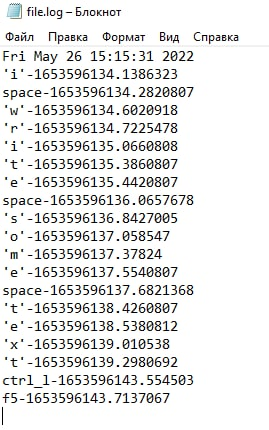
\includegraphics[width=0.6\textwidth]{photo/kl1.png}
    \caption{Содержимое файла file.log}
    \label{r1}
  \end{figure}

  Далее опять запускается данная программа, но уже тот же самый текст набирает \textit{пользователь 2}. И в итоге получается новый файл file1.log,
  как показано на рисунке \ref{r2}. 



  \begin{figure}[H]
    \centering
    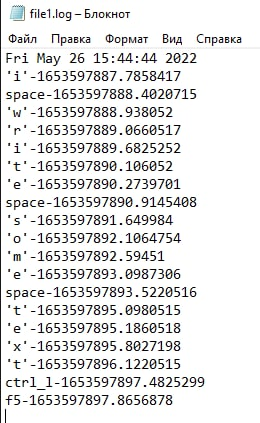
\includegraphics[width=0.6\textwidth]{photo/kl2.png}
    \caption{Содержимое файла file1.log}
    \label{r2}
  \end{figure}

  Затем эти файлы отправляются на анализ для построения гистограммы. На рисунке \ref{analyze} изображен ввод данных, где программа
  запрашивает у пользователя количество файлов для анализа, их имена, а также дает возможность построить гистограмму для любых двух
  заданных файлов.
  
  
  \begin{figure}[H]
    \centering
    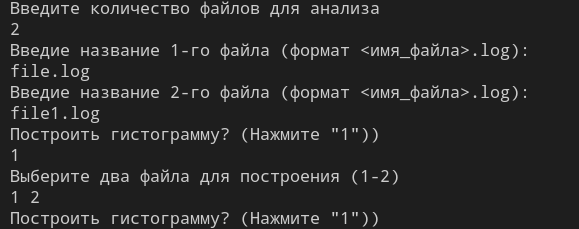
\includegraphics[width=0.7\textwidth]{photo/analyze.png}
    \caption{Ввод данных для анализа}
    \label{analyze}
  \end{figure}
  
  На рисунке \ref{hist} показана диаграмма, в которой можно увидеть разницу пауз нажатия клавиш.

  \begin{figure}[H]
    \centering
    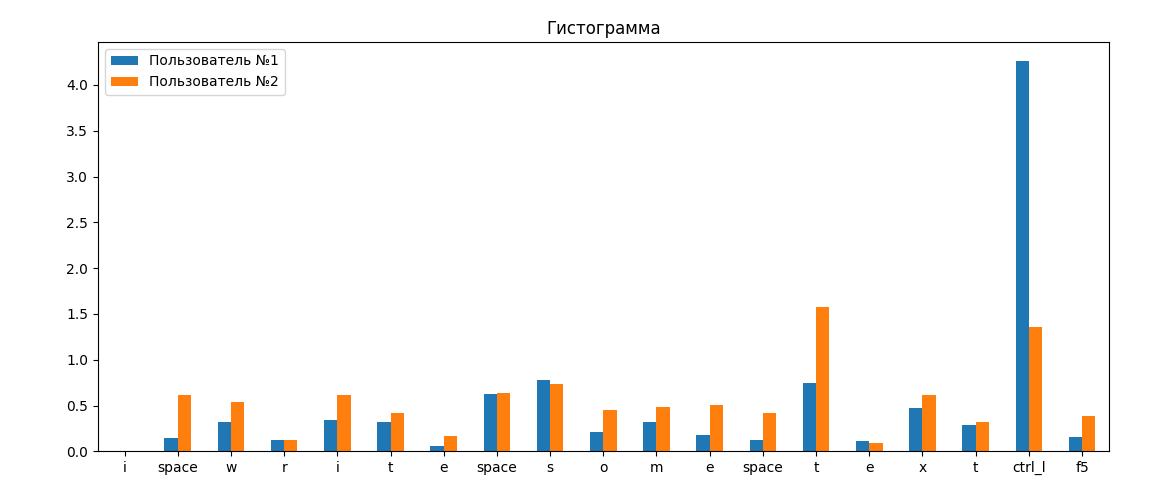
\includegraphics[width=0.8\textwidth]{photo/hist.png}
    \caption{Гистограмма}
    \label{hist}
  \end{figure}

  Можно сделать вывод, что паузы нажатия клавиш, между \textit{пользователем 1} и \textit{пользователем 2} различаются. Но всё таки эту разницу
  возможно свести к минимуму, если \textit{пользователь 2} постарается подделать почерк \textit{пользователя 1}. Поэтому такой подход будет считаться
  ненадежным и бессмысленным.

   \conclusion

  В данной работе был рассмотрен протокол RDP\dots

  \begin{thebibliography}{15}
    \bibitem{1}
    Книга Ибе О.С. «Компьютерные сети и службы удаленного доступа» / пер. с англ. -
    Москва, издательство: «ДМК Пресс», Яз. рус.
    \bibitem{2}
    Удалённый рабочий стол RDP: как включить и как подключиться по RDP [Электронный ресурс] / URL:https://hackware.ru/?p=11835 (дата обращения 03.05.2022), Яз. рус.
    \bibitem{3}
    Документация по устранению неполадок служб удаленных рабочих стола для Windows Server [Электронный ресурс] / URL: https://inlnk.ru/bvOV0 (дата обращения 04.05. 2022), Яз. рус.

  \end{thebibliography}

  \appendix

    \section{Код keylogger-win.py}
    \inputminted[fontsize=\footnotesize]{text}{keylogger-win.py}

    % \section{Код keylogger-linux.py}
    % \inputminted[fontsize=\footnotesize]{text}{keylogger-linux.py}

    \section{Код analyze-data.py}
    \inputminted[fontsize=\footnotesize]{text}{analyze-data.py}

\end{document}